\section{Justificación del trabajo de grado}
En todos los ámbitos de la vida de las personas como la educación, la economía, la política, la cultura y el medio ambiente. Estas transformaciones sociales a nivel mundial generan acciones de aprendizajes y de mercados globales, donde las tecnologías y los aportes de nuevos o mejorados software “generan reducciones significativas de costos por la experiencia y utilización de patentes o porque aportan beneficios por la capacidad de vender variedades similares de productos en diversos mercados” \citep[p. 27]{vela2012}.

En la actualidad, la agricultura es un renglón económico que viene identificando diseños de políticas públicas para la intervención de aplicaciones tecnológicas y generar el aprovechamiento y mejoras de la productividad agraria a nivel mundial. Estas iniciativas resultan de las dificultades económicas y de productividad agraria, las cuales deben de ser transformadas para el desarrollo del campo, como explica la FAO (\citeyear{fao2021}):

\begin{quote}
    La incorporación de estas tecnologías supone la generación de información (basada en la recopilación y procesamiento de datos) e indicaciones que permiten el monitoreo, el análisis, la planificación y el control inteligente de procesos de producción, transformación, distribución y comercialización de productos agrícolas \cite[p.88]{fao2021}.
\end{quote}


El uso de tecnología y datos se ha vuelto cada vez más importante para mejorar la eficiencia y la productividad en la agricultura. En este contexto, el empleo de la metodología MLOps (Machine Learning Operations) se justifica como una herramienta poderosa para potenciar la agricultura y lograr una gestión más eficiente de los recursos. Estas mejoras en América Latina proporcionan una sostenibilidad en la producción agrícola y contribuye a procesos más saludable para el medio ambiente (ver figura \ref{fig:figura1}).

\begin{figure}[h]
\centering
\caption{Acceso y aprovechamiento de tecnología digital en la agricultura de América del Sur}
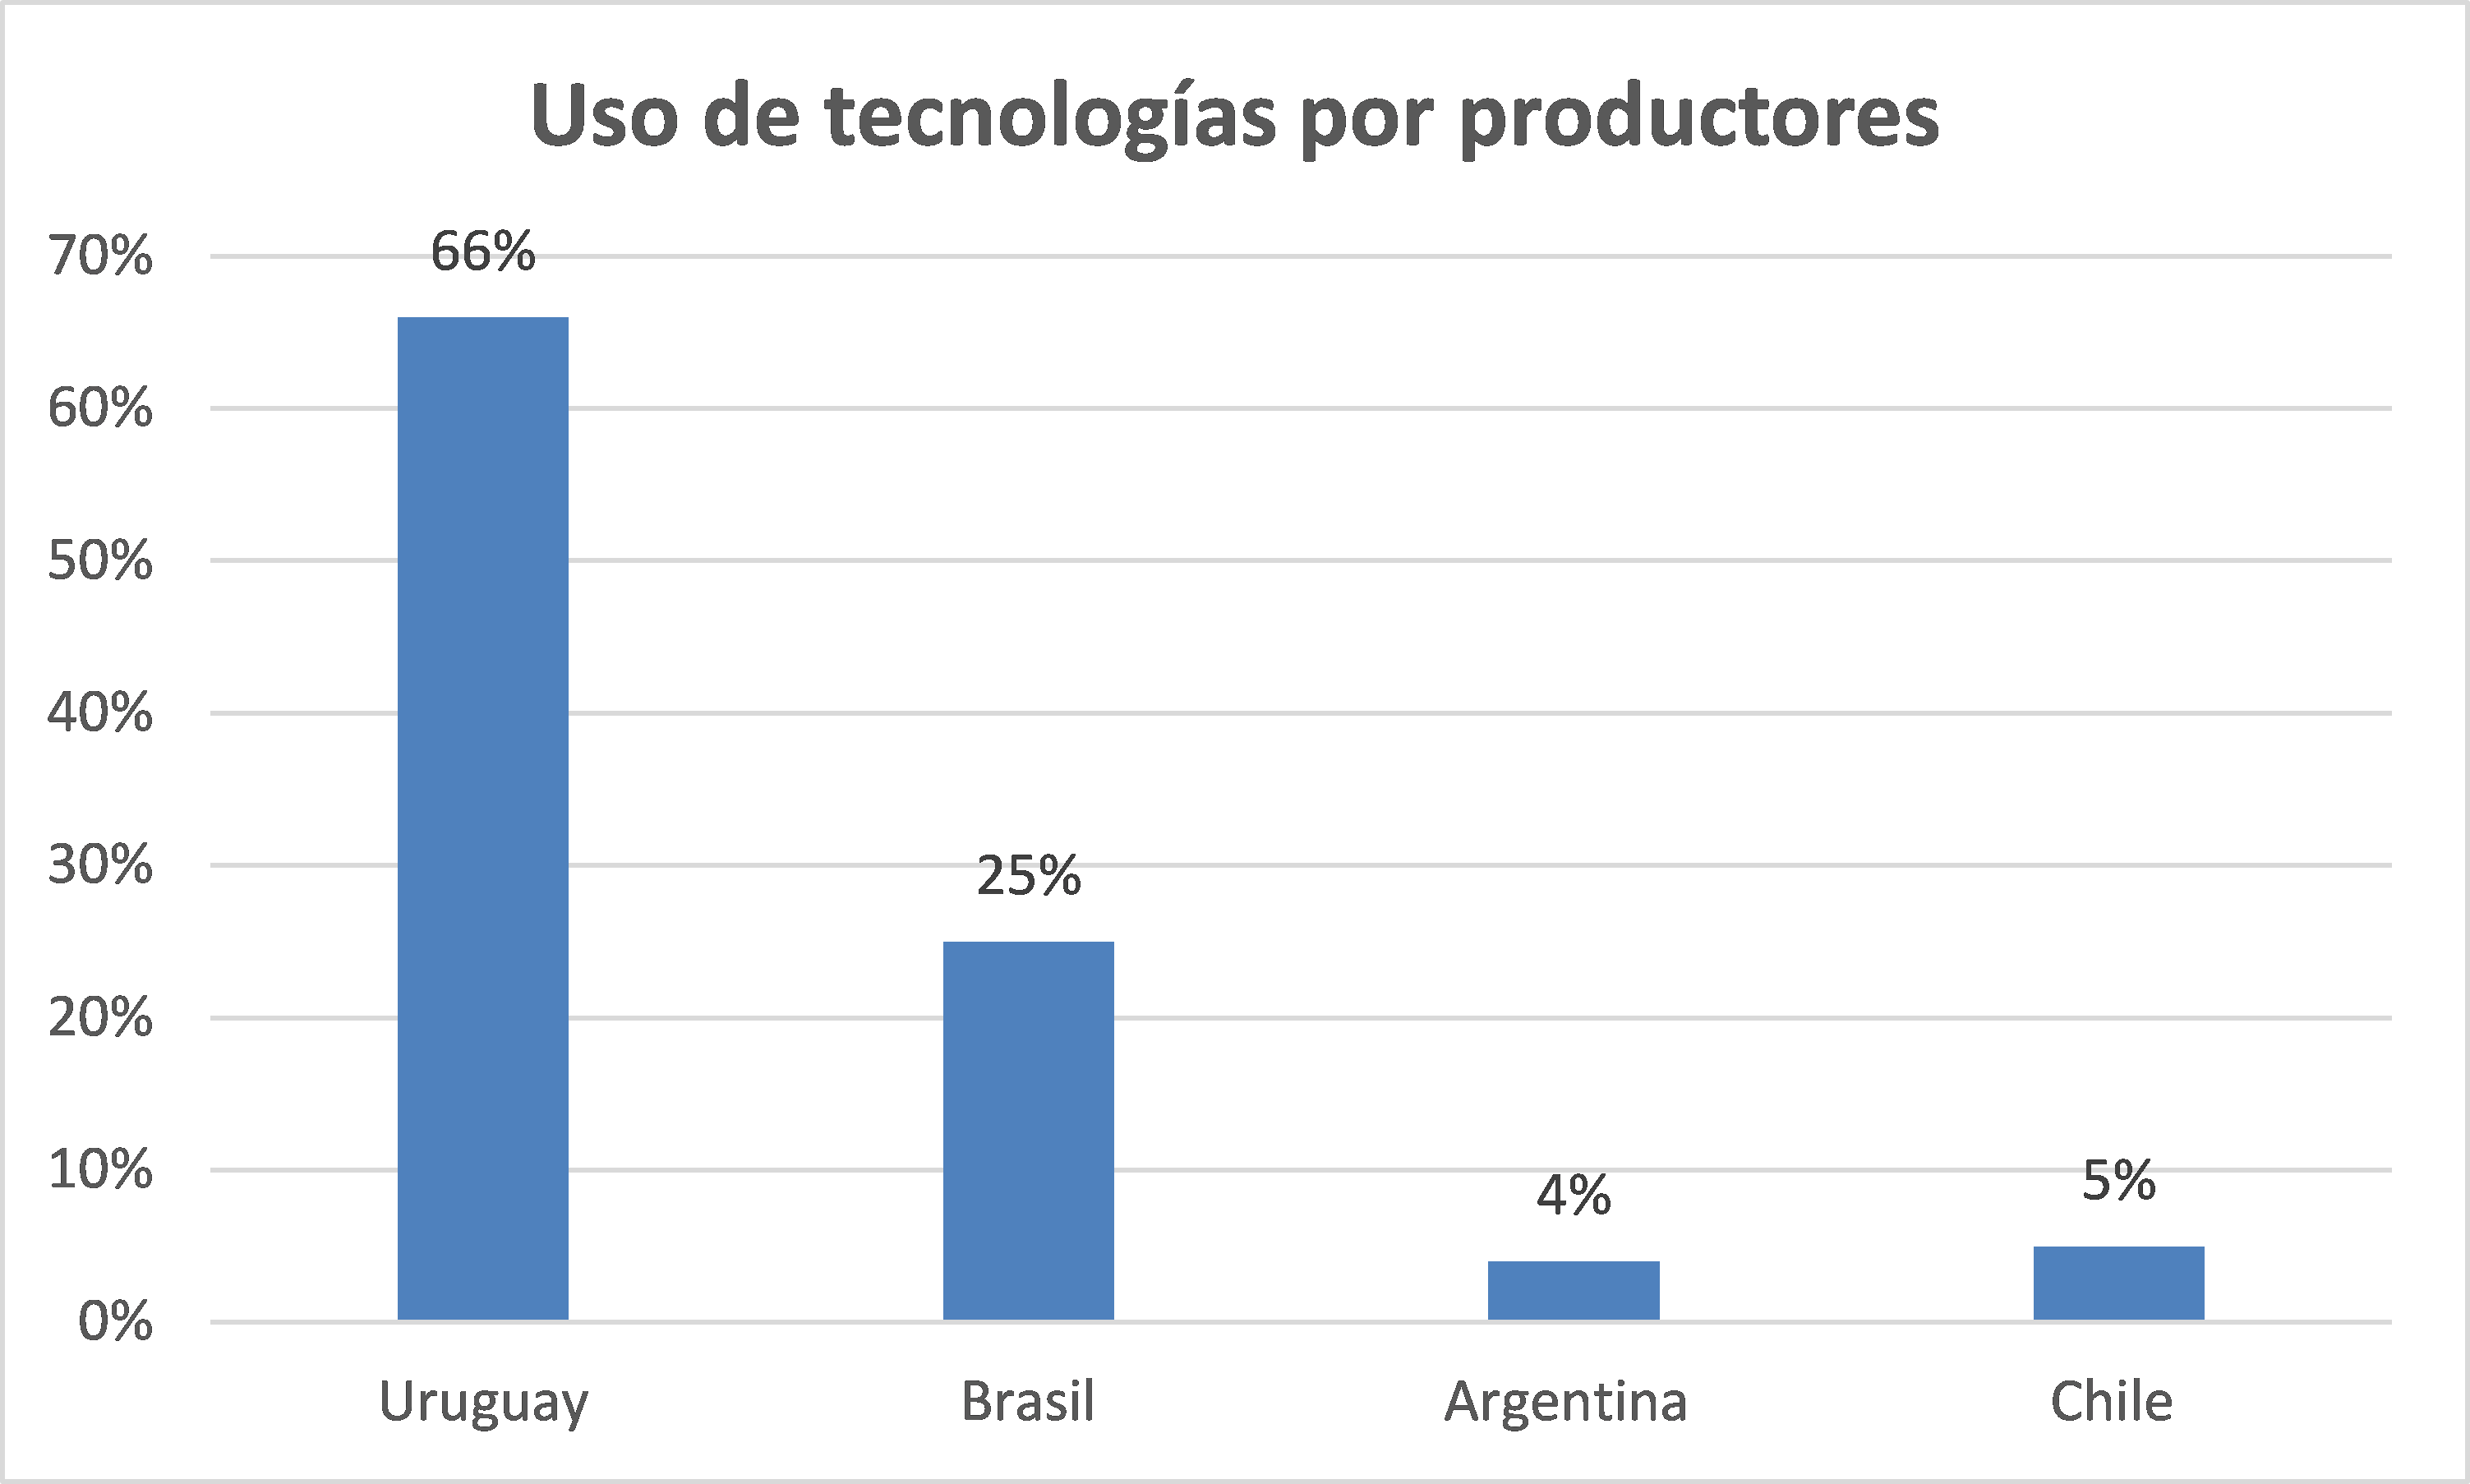
\includegraphics[width=1\textwidth]{usoTecnologias.png}
\caption*{\footnotesize Fuente: Información tomada de FAO \citeyear{fao2021}}
\label{fig:figura1}
\end{figure}

\newpage

El uso de la metodología MLOps en la agricultura ofrece mejoras debido a su capacidad para optimizar la toma de decisiones, automatizar tareas y mejorar la precisión de los resultados de los modelos de machine learning. Esta tecnología puede marcar una gran diferencia en la eficiencia y la sostenibilidad de la agricultura, ayudando a enfrentar los desafíos actuales y futuros del sector.

De allí que, la metodología MLOps tiene un gran potencial para transformar la agricultura y brindar beneficios significativos a los científicos de datos involucrados en esta industria, debido a que pueden aprovechar varias ventajas, como por ejemplo el MLOps permite una mejor gestión de los modelos de aprendizaje automático, es posible utilizar prácticas de control de versiones para rastrear y gestionar los cambios en los modelos, lo que facilita la colaboración y la reproducibilidad de los resultados en las áreas de producción agrícola. Además, el MLOps garantiza un monitoreo continuo de los modelos en producción, lo que permite identificar y solucionar problemas rápidamente.

Al utilizar técnicas de aprendizaje automático, los científicos de datos pueden analizar grandes volúmenes de datos agrícolas para identificar patrones y tomar decisiones informadas, ayudando a implementar estos modelos en sistemas integrados, lo que permite la automatización de tareas agrícolas como el riego, la fertilización y la detección de enfermedades. Esto conduce a un uso más eficiente de los recursos, reduciendo costos y minimizando el impacto ambiental.

En este sentido la tecnología constituye una herramienta relevante para el mundo actual, de allí que este tipo de investigaciones permitan abordar métodos aplicables en la ingeniería de software tanto para la generación de conocimientos, como métodos de aplicación en escenarios reales, como la agricultura y, en particular, el cultivo del aguacate Hass. Asimismo, esta clase de investigaciones abre la vía para la articulación entre los profesionales, las universidades y la industria agrícola para fomentar prácticas económicas y tecnológicas, mejorar y fortalecer actividades de investigación en laboratorios de computación y programas de alfabetización digital, con el objetivo de contribuir al desarrollo económico, científico y académico, asegurando que la ingeniería de software se emplee de forma concreta y provechosa en la solución de problemas prácticos en diversas áreas, como la agricultura.